% Chapter 6: Morphological Relations, Convergence, and Divergence

\section{Static Similarity Across Fields}

Chapters 4 and 5 compared field profiles one by one. This chapter compares fields directly with each other. Morphological similarity means Euclidean closeness between robust-scaled field profiles built from the same eight structural metrics. Low distance means similar dispersion, local density, hubness, and spectral structure. It is not semantic similarity: fields may have similar shape while studying different topics.

\begin{figure}[H]
\centering
\caption[Pairwise field morphological distances]{Pairwise morphological distance between fields using the eight structural metrics. Lower values indicate more similar robust-scaled morphology profiles.}
\label{fig:field_static_distance_heatmap}
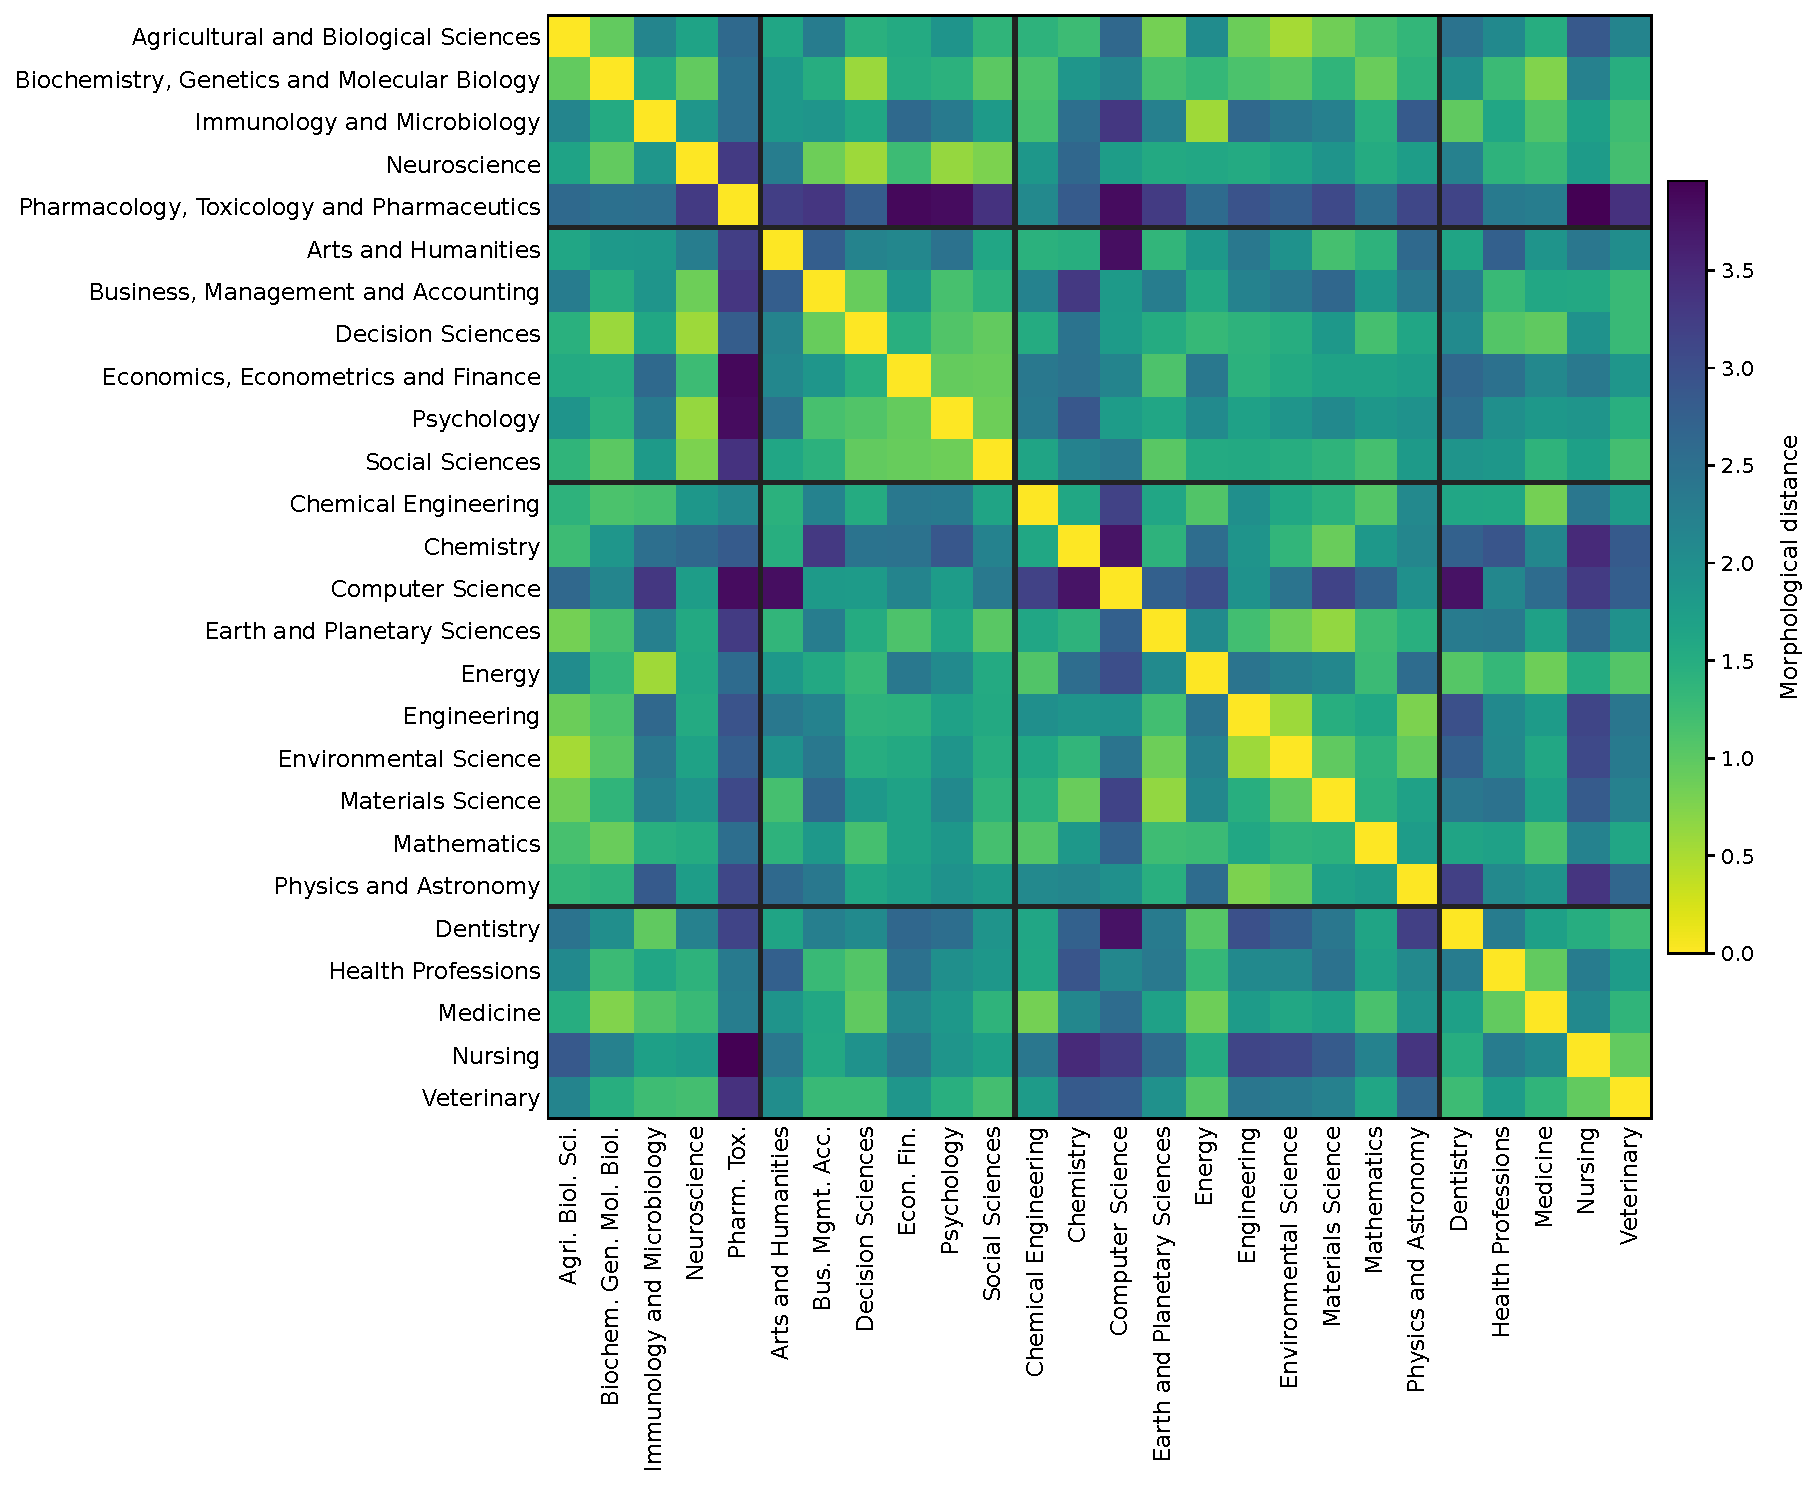
\includegraphics[width=\textwidth]{figures/fig_06_field_static_distance_heatmap.pdf}
\end{figure}

The closest pairs are mostly cross-domain. The minimum is Agricultural and Biological Sciences with Environmental Science (\(0.530\)), followed by Energy with Immunology and Microbiology (\(0.562\)) and Decision Sciences with Neuroscience (\(0.575\)). These distances indicate similar structural profiles, not shared content.

\section{Taxonomy, Bridges, and Isolates}

The domain-pair summary gives a useful contextual check. Within-domain field pairs have a lower median distance than cross-domain pairs, \(1.62\) versus \(1.86\). Taxonomy therefore still matters. However, the relationship is uneven. Social Sciences are the most internally coherent domain, and the closest cross-domain medians involve Life Sciences with Social Sciences and Life Sciences with Physical Sciences. At field level, 17 of 26 fields have their nearest morphological neighbor outside their own domain.

\begin{figure}[H]
\centering
\caption[Domain-pair morphological distance structure]{Domain-pair morphological distance structure. Panel A reports median field-pair distances by OpenAlex domain pair; Panel B counts within-domain and cross-domain nearest neighbors.}
\label{fig:domain_pair_distance_structure}
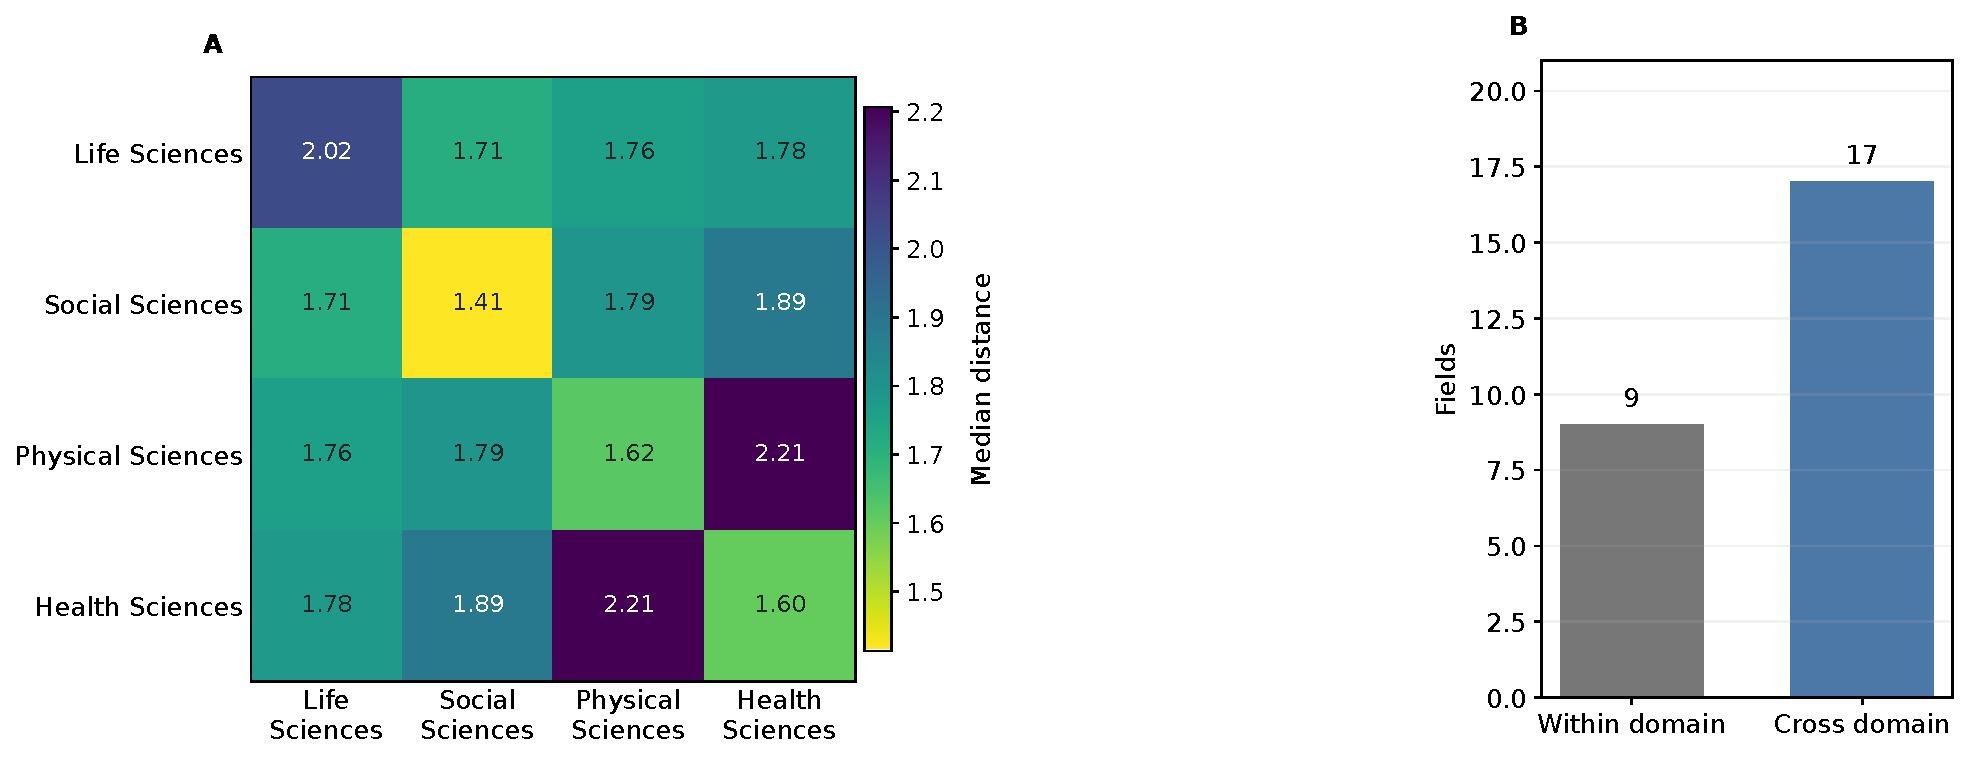
\includegraphics[width=\textwidth]{figures/fig_06_domain_pair_distance_structure.pdf}
\end{figure}

The idea of a bridge is useful here because it shows where taxonomy and morphology do not fully coincide. Some fields sit near a field from another domain because their document clouds have a similar balance of compactness, dispersion, local density, and spectral structure. The result is not a failure of the OpenAlex taxonomy. It is a reminder that a field can belong to one administrative domain while having a structural profile closer to another part of the map.

The isolates are equally informative. Pharmacology, Toxicology and Pharmaceutics has the largest nearest-neighbor distance, with Chemical Engineering still \(2.10\) away. Computer Science follows, with Neuroscience \(1.75\) away. These fields are not isolated because they lack scientific relations in general. They are isolated because their eight-metric morphology profile has no very close field-level neighbor in this representation.

\section{Convergence and Divergence}

Temporal convergence and divergence use the eight structural metrics inside each five-year window. A pair converges when the distance between its two field profiles decreases from 2000--2004 to 2020--2024, and diverges when it increases. Centroid drift is excluded because it measures movement of the field center, not structural profile distance.

This use of changing profile distance is connected to science-mapping work on evolving interdisciplinarity and network coherence \parencite{porter2009interdisciplinary,rafols2010networkcoherence,leydesdorff2011indicators}. The interpretation remains descriptive. Convergence means that two field profiles become more similar under the selected metrics; it does not prove collaboration, integration, or causal influence.

The temporal picture is not global convergence. Across all 325 field pairs, mean Euclidean distance rises from \(1.44\) in 2000--2004 to \(1.81\) in 2020--2024. The same upward movement appears within domains, from \(1.39\) to \(1.70\), and across domains, from \(1.46\) to \(1.85\). Field-level morphology space becomes more separated on average, even though many individual pairs move closer.

\begin{figure}[H]
\centering
\caption[Temporal field-pair distance trajectories]{Mean field-pair morphological distance across five-year windows using the eight windowed structural metrics.}
\label{fig:temporal_distance_trajectories}
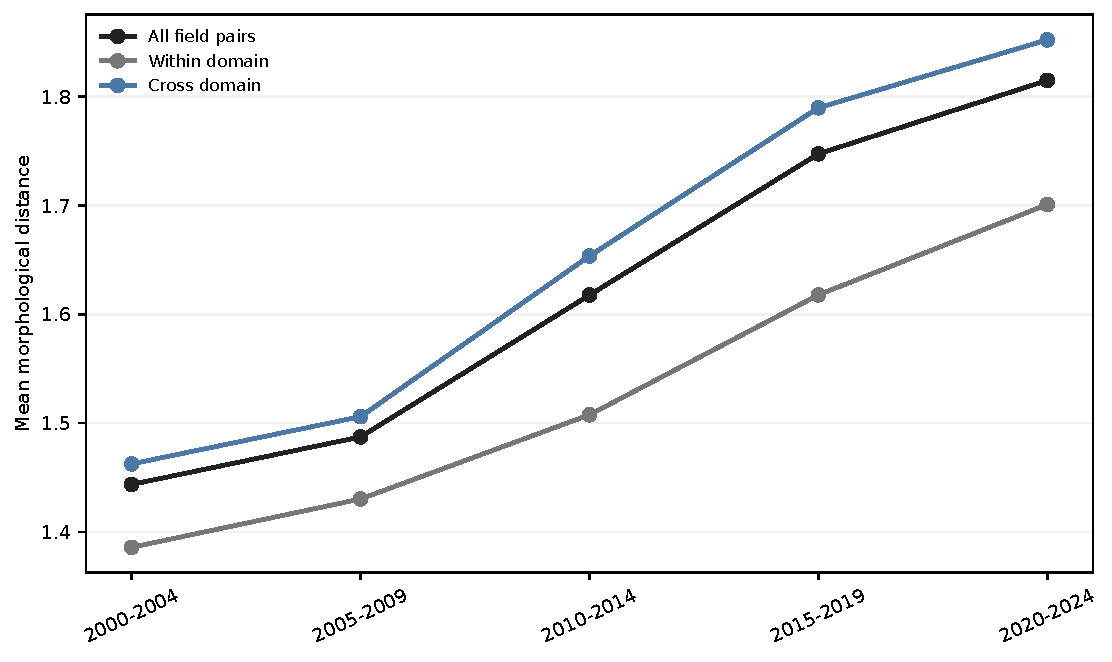
\includegraphics[width=0.88\textwidth]{figures/fig_06_temporal_distance_trajectories.pdf}
\end{figure}

Selective convergence remains visible: 97 field pairs decrease in distance, while 228 increase. The strongest convergences tend to involve shared declines in local distance and spectral dimensionality. Materials Science and Mathematics move from \(1.75\) to \(0.85\). Decision Sciences and Environmental Science move from \(1.67\) to \(0.82\). Economics, Econometrics and Finance and Psychology move from \(1.53\) to \(0.70\). The diverging side has a clearer protagonist: Computer Science appears in nine of the ten largest field-level Euclidean divergences.

This combination is important. The mean curve in Figure~\ref{fig:temporal_distance_trajectories} moves upward, so the general direction is separation. However, the pair-level ranking shows that separation is not uniform. Some pairs move closer because they share the same kind of structural change. Other pairs move apart because one field changes in a different metric family. Figure~\ref{fig:field_convergence_divergence_pairs} makes this asymmetry visible.

\begin{figure}[H]
\centering
\caption[Strongest field-level convergence and divergence pairs]{Strongest field-level convergence and divergence under Euclidean profile distance. Open markers are initial distances and filled markers are final distances; labels show final-minus-initial change.}
\label{fig:field_convergence_divergence_pairs}
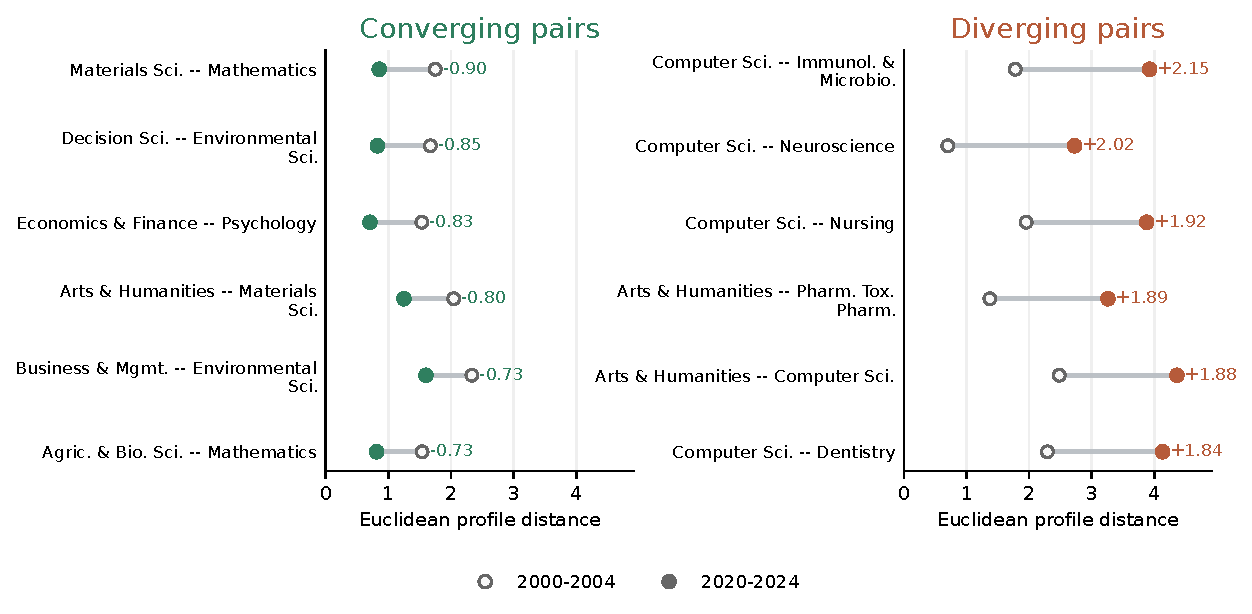
\includegraphics[width=\textwidth]{figures/fig_06_field_convergence_divergence_pairs.pdf}
\end{figure}

The same distance change can come from different metric movements. Some convergences reflect both fields becoming locally denser or lower-dimensional. Some divergences occur because one field changes sharply while the other follows the population average. Computer Science is the clearest case. Its large drops in PCA dimensionality and spectral entropy separate its windowed profile from many fields that also become locally denser but do not move in the same spectral direction.

The direct answer to the third research question comes primarily from the temporal pairwise distances. Mean field-pair morphological distance increases from 1.44 in 2000--2004 to 1.81 in 2020--2024. In total, 228 of the 325 field pairs diverge, while 97 converge. The strongest converging pairs are Materials Science with Mathematics, Decision Sciences with Environmental Science, and Economics, Econometrics and Finance with Psychology. The strongest divergences include Computer Science with Immunology and Microbiology, Neuroscience, and Nursing.

OpenAlex-domain alignment, cross-domain nearest neighbors, bridges, and isolates remain useful complementary context. They show that field relations partly cross taxonomy. The main evidence for Research Question 3, however, is the observed increase, convergence, and divergence of structural profile distances over time.
